\section{子问题一：月度能源消耗量预测}

\subsection{问题定义与难点}

任务一的目标是基于消费者的出行与车辆特征，预测其每月的电动汽车能源消耗量 monthly\_energy\_consumption\_kwh。电力公司可据此预测电动汽车接入电网后的负荷。评分指标为调整决定系数 adj-$R^2$。

题面提示的核心难点是``该指标与行驶距离强相关，但受驾驶习惯和车型影响，需挖掘 daily\_commute\_km 与 vehicle\_type 的交互特征''。然而，数据探索阶段的比率诊断已表明，月能耗与周里程之间近似比例关系，且``单位里程能耗''这一随机量几乎不随车型或驾驶习惯变化。

\subsection{探索性数据分析}

\subsubsection{周里程与能耗的线性关系}

如图\ref{fig:t1_scatter}所示，月能耗随周里程线性增长，散点沿一条通过原点的直线均匀分布。以周里程的比率均值模型（$energy = r \cdot weekly$，其中 $r = \mathrm{mean}(energy/weekly)$）拟合，折外 adj-$R^2$ 即达 0.876300。

\begin{figure}[H]
\centering
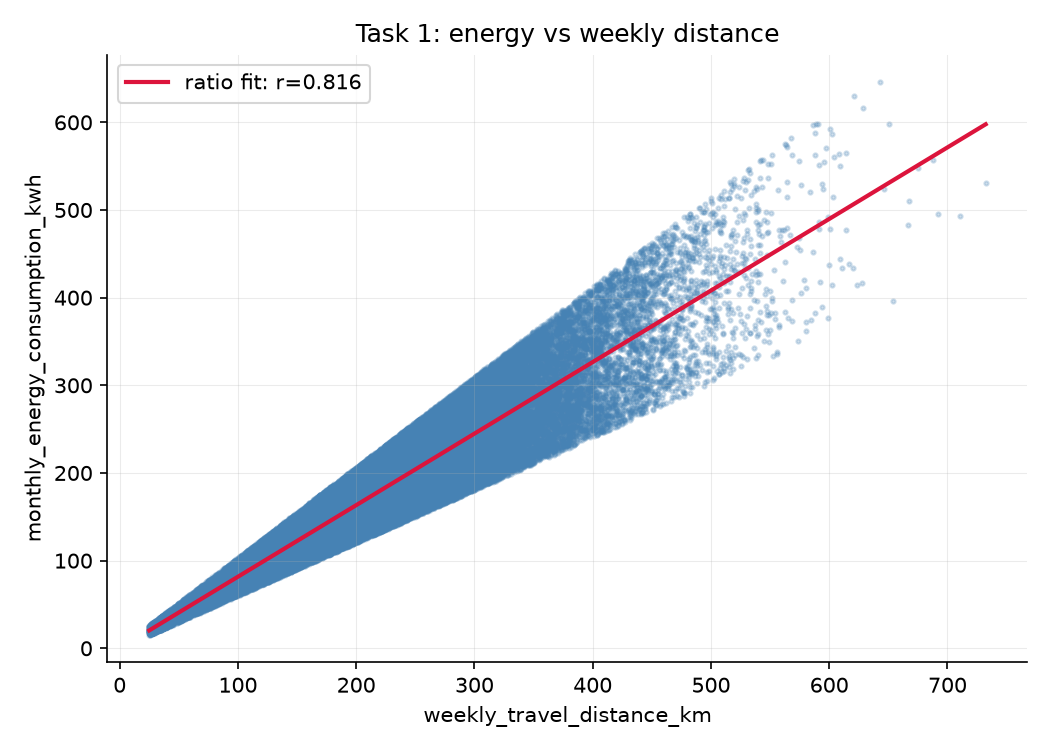
\includegraphics[width=0.8\textwidth]{figures/task1_energy_scatter.png}
\caption{月能耗与周行驶里程散点图及比率拟合线}
\label{fig:t1_scatter}
\end{figure}

\subsubsection{单位里程能耗的分布}

图\ref{fig:t1_ratio}给出单位里程能耗 $energy/weekly$ 的分布，近似为 0.60--1.03 区间内的平坦分布。该比率与所有可观测输入的相关系数绝对值均低于 0.01，各车型的平均值差异不足 0.001。这说明``能效''在当前数据中是一个与特征无关的随机量，模型能够解释的部分几乎全部来自周里程本身。

\begin{figure}[H]
\centering
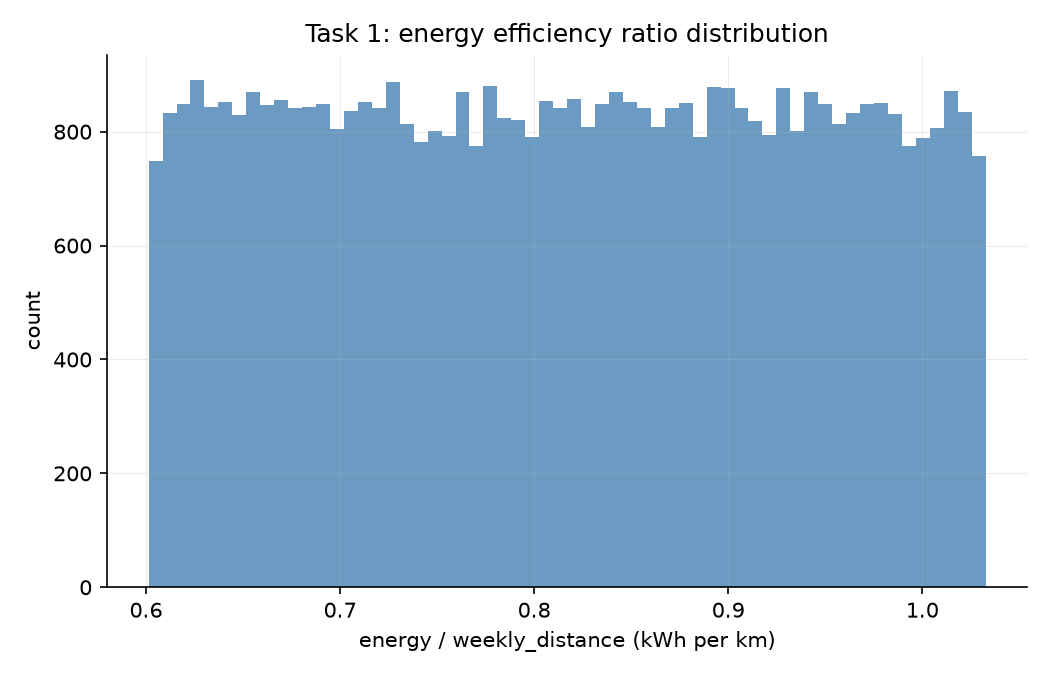
\includegraphics[width=0.8\textwidth]{figures/task1_ratio_dist.png}
\caption{单位里程能耗比率分布}
\label{fig:t1_ratio}
\end{figure}

\subsection{模型选择与消融}

\subsubsection{稀疏基线对比}

任务一首先比较三种稀疏基线：比率均值模型、过原点 OLS、带截距 OLS。结果如表\ref{tab:t1_baseline}所示，三者性能几乎一致，比率均值模型以 adj-$R^2=0.876300$ 略优，且具有最强的业务解释力。

\begin{table}[H]
\centering
\caption{任务一稀疏基线对比（5 折 OOF）}
\label{tab:t1_baseline}
\begin{tabular}{lccc}
\toprule
\textbf{模型} & \textbf{$R^2$} & \textbf{adj-$R^2$} & \textbf{RMSE} \\
\midrule
比率均值（$r\cdot weekly$） & 0.876302 & \textbf{0.876300} & 31.04 \\
过原点 OLS & 0.876296 & 0.876293 & 31.04 \\
带截距 OLS & 0.876290 & 0.876288 & 31.04 \\
\bottomrule
\end{tabular}
\end{table}

\subsubsection{特征块消融}

本文进一步验证题面建议的特征方向是否有效。以周里程为核心，逐块加入行程结构、官方车型交互、车辆/地域与其他信息特征，结果如表\ref{tab:t1_ablation}所示。

\begin{table}[H]
\centering
\caption{任务一特征块消融结果（adj-$R^2$）}
\label{tab:t1_ablation}
\begin{tabular}{lcc}
\toprule
\textbf{特征组合} & \textbf{特征数} & \textbf{adj-$R^2$} \\
\midrule
F0 核心（周里程） & 1 & \textbf{0.876300} \\
F0 + 行程结构 & 4 & 0.876277 \\
F0 + 官方车型交互 & 7 & 0.876271 \\
F0 + 车辆/地域 & 7 & 0.876244 \\
F0 + 其他信息 & 20 & 0.876198 \\
全特征 & 35 & 0.876149 \\
\bottomrule
\end{tabular}
\end{table}

消融结果与数据生成机制完全一致：任何特征块的加入都使 adj-$R^2$ 下降，官方提示的``里程 $\times$ 车型''交互无任何增益。原因在于 adj-$R^2$ 对新增预测变量施加自由度惩罚，而无增益特征只会增加模型复杂度。最终模型确定为单变量比率均值模型。

\subsection{残差诊断与非线性确认}

为验证稀疏模型是否已充分拟合，本文在基线的折内残差上训练浅层 LightGBM，观察其能否解释残差中的剩余结构。结果如表\ref{tab:t1_tree}所示：树模型相对基线的 $\Delta R^2$ 为 $-0.001430$，Bootstrap 95\% 置信区间为 $[-0.001799, -0.001070]$，整体小于 0。树模型不仅无增益，反而因拟合噪声而变差。

\begin{table}[H]
\centering
\caption{任务一树模型残差确认}
\label{tab:t1_tree}
\begin{tabular}{lccc}
\toprule
\textbf{方案} & \textbf{$R^2$} & \textbf{$\Delta R^2$（Bootstrap 95\% CI）} & \textbf{结论} \\
\midrule
稀疏基线 & 0.876300 & -- & 主方案 \\
残差 LightGBM & 0.874881 & $[-0.001799, -0.001070]$ & 淘汰 \\
\bottomrule
\end{tabular}
\end{table}

\subsection{最终模型}

任务一的最终模型为：

\begin{equation}
\hat{y}_1 = r_1 \cdot weekly\_travel\_distance\_km, \quad r_1 = 0.8163487
\label{eq:t1}
\end{equation}

在 5 折 $\times$ 3 种子最终确认中，adj-$R^2$ 均值为 0.876298 $\pm$ 0.000007，折间标准差极小，模型高度稳定。
